\chapter{Results and Analysis}
\label{chapter:results-analysis}
	
	In this chapter, we begin an analysis of 1D heterogeneous systems, then move our attention to 2D heterogeneous systems. Although 1D homogeneous systems were simulated, they did not provide any interesting or new insight into diffusive behaviour, therefore those simulations and analytical data are not presented in detail. We begin each section with selected images of simulated density distributions to motivate further analysis. More specifically, we analyze how changing the boundary transition probabilities, region diffusivities, and cell geometry (2D only), affects the mean-squared-displacement (MSD) and show that sub- and super-diffusive regimes exist. Lastly, we show that the long-time effective diffusivity is non-trivial even for simple-cell geometries.
	
\section{1D Systems}
\label{sec:ra-1D}
	For very large systems or short simulation times---conditions where the density distribution is zero at the absolute boundaries---agreement between the Monte Carlo (MC) and master equation (ME) simulation solutions, and analytical solutions (\ref{eq:1D-diffusion-equation-solution}) of the 1D diffusion equation with no net drift and constant diffusion factor (\ref{eq:1D-diffusion-equation}), was observed (Figure \ref{fig:11U_homogeneous_plots_1D}). 

	\begin{figure}[h]
		\centering
		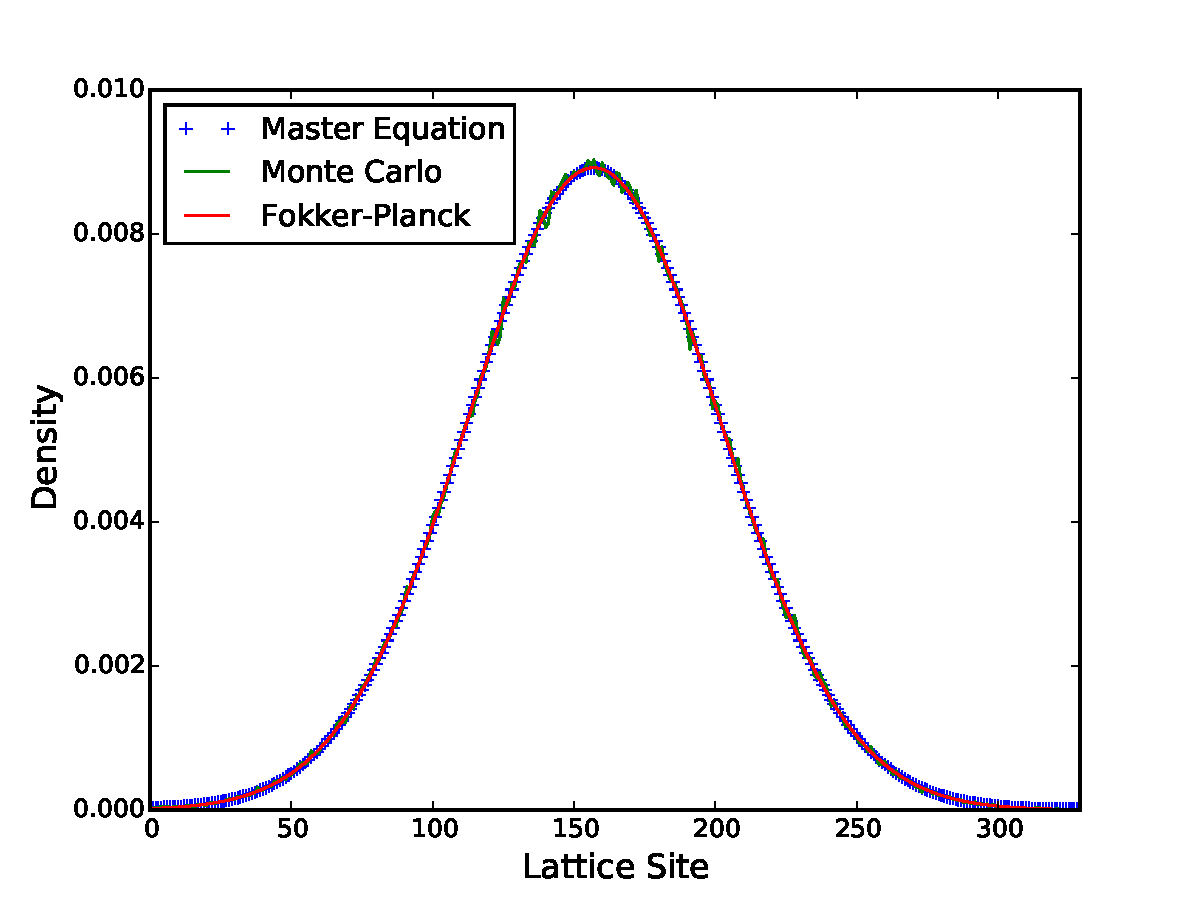
\includegraphics[width=1.0\linewidth]{../images/1D/11U_homogeneous_plots_1D}
		\caption{Simple 1D system with no internal semi-permeable boundaries. Simulation solutions plotted for ME and MC methods. Additionally, an exact solution to diffusion equation (Fokker-Planck) is plotted. Parameter specifications: 330 lattice sites, $ D = 0.1 $, $ N = 8\cdot10^5 $ particles in MC simulation, and density normalized.}
		\label{fig:11U_homogeneous_plots_1D}
	\end{figure}
	
	\nointerlineskip The 1D diffusion equation \ref{eq:1D-diffusion-equation} may be known as a `simple' Fokker-Planck or Smoluchowski equation and is sometimes utilized as a model of classical Brownian motion.
	
	\begin{equation}
	\label{eq:1D-diffusion-equation}
		\frac{\partial\rho(x,t)}{\partial t} = D_0 \frac{\partial^2 \rho(x,t)}{\partial x^2}
	\end{equation}
	
	Assuming that $ N $ particles start from the origin, Equation \ref{eq:1D-diffusion-equation} has the solution:
	
	\begin{equation}
	\label{eq:1D-diffusion-equation-solution}
		\rho(x,t)=\frac{N}{\sqrt{4\pi Dt}}e^{-\frac{x^2}{4Dt}}
	\end{equation}	
	
	A variant of Equation \ref{eq:1D-diffusion-equation-solution} was used to create the Fokker-Planck plot in Figure \ref{fig:11U_homogeneous_plots_1D}. The solution to \ref{eq:1D-diffusion-equation} is not a solution to a boundary value problem. For example, it is possible to solve \ref{eq:1D-diffusion-equation} for reflecting absolute boundary conditions: $ \rho_x(0,t) = \rho_x(L,t) = 0 $. It is even possible to solve it for `repeating' boundary conditions that represent semi-permeable internal boundaries (Jessica Cervi's thesis); these specific problems were not explored and are not discussed further. However, it is comparatively easy to obtain a solution to such a system with internal semi-permeable and absolute reflecting boundaries by utilizing MC and ME methods for the simulation of the system; Figure \ref{fig:11U_heterogeneous_plots_1D} shows such a solution.
	
	With reference to Figure \ref{fig:11U_homogeneous_plots_1D}, note the good agreement between the ME and MC simulation solutions and analytical solution. The ME simulation solution and analytical solution are perfectly superimposed. The MC simulation shows characteristic statistical fluctuations that reflect the underlying `random' movement of individual particles in the simulation. The relative magnitude of these fluctuations decreases with an increasing number of particles $ N $ according to $ 1/\sqrt{N} $.

	\begin{figure}[h]
		\centering
		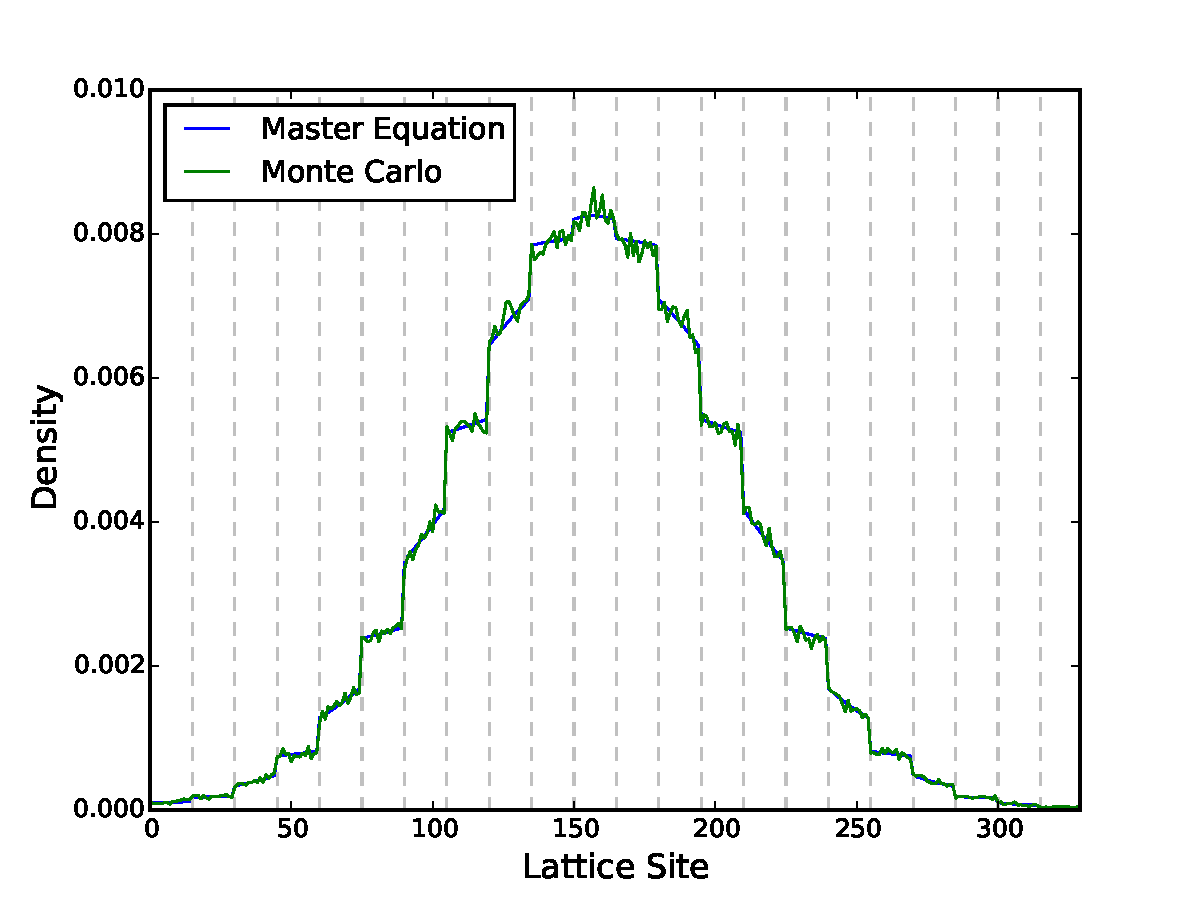
\includegraphics[width=1.0\linewidth]{../images/1D/11U_heterogeneous_plots_1D}
		\caption{1D heterogeneous system with internal semi-permeable boundaries. Simulation solutions plotted for ME and MC methods. Parameter specifications: 330 lattice sites, 15 lattice sites per cellular or extracellular region, $ D_i = 0.05 $, $ D_e = 0.2 $, and $ P_{i\rightarrow e} = 0.05 $. $ N = 5 \cdot 10^5 $ particles in the MC simulation and density normalized. Vertical dashed lines show semi-permeable boundary positions.}
		\label{fig:11U_heterogeneous_plots_1D}
	\end{figure}
	
	Statistical fluctuations in the MC simulation solution are more visible in Figure \ref{fig:11U_heterogeneous_plots_1D}. The ME simulation was orders of magnitude faster in reaching completion and does not show any fluctuations since the density distribution is evolved in time under the assumption that there are \textsl{very} many particles at each lattice site. It is expected that in the limit of an infinite number of particles, the MC solution converges to the ME solution. Comparisons to analytical or numerical solutions of the Fokker-Planck equation were not made but doing so may be of interest in the future.
	
	\begin{figure}[h]
		\centering
		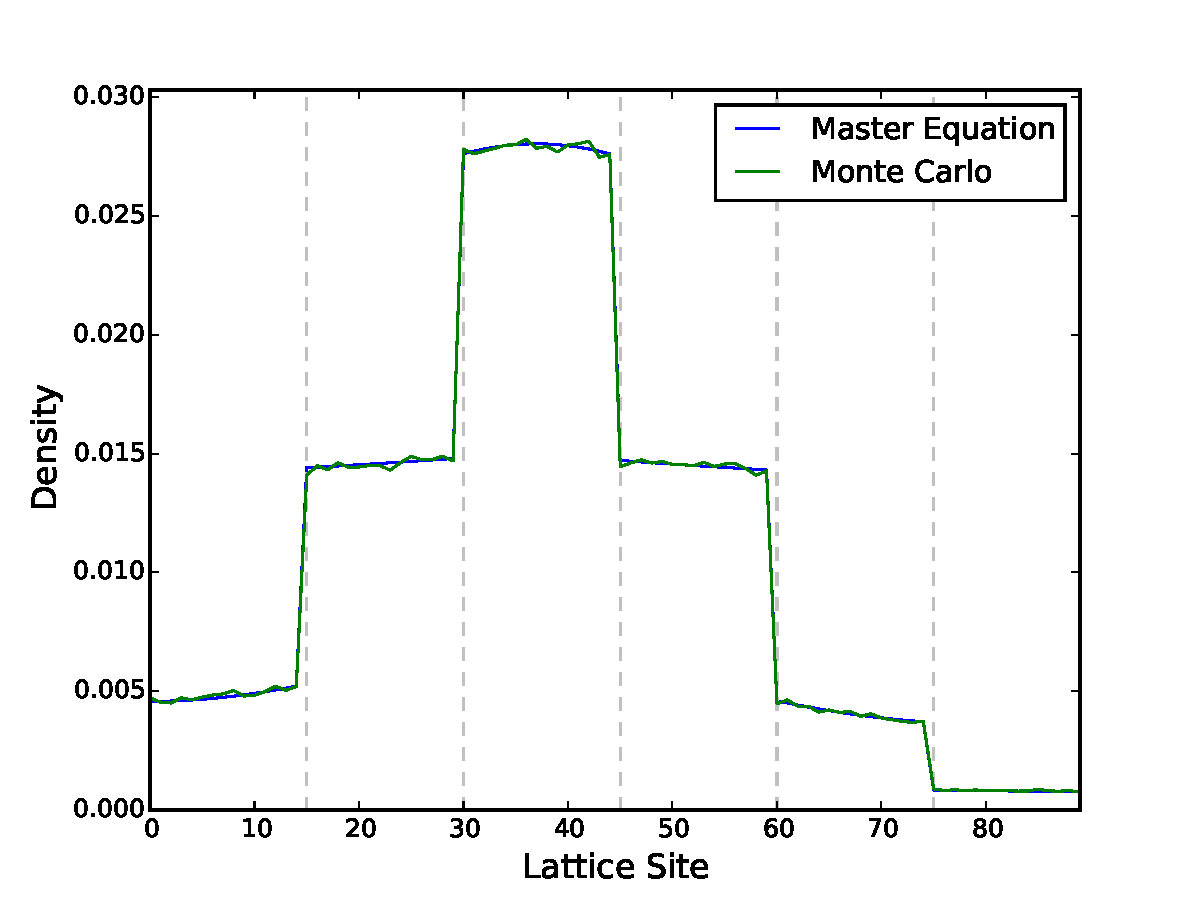
\includegraphics[width=1.0\linewidth]{../images/1D/3U_heterogeneous_plots_1D}
		\caption{1D heterogeneous system with internal semi-permeable boundaries. Simulation solutions plotted for ME and MC methods. Parameter specifications: 90 lattice sites, 15 lattice sites per cellular or extracellular region, $ D_i = 0.05 $, $ D_e = 0.2 $, and $ P_{i\rightarrow e} = 0.01 $. $ N = 8 \cdot 10^5 $ particles in the MC simulation and density normalized. Vertical dashed lines show semi-permeable boundary positions.}
		\label{fig:3U_heterogeneous_plots_1D}
	\end{figure}
	
	\newpage
	Interesting to note in Figure \ref{fig:11U_heterogeneous_plots_1D} and \ref{fig:3U_heterogeneous_plots_1D}, the magnitude of the fluctuations in the MC solution appear larger at higher densities and smaller at lower densities. In Figure \ref{fig:11U_heterogeneous_plots_1D}, extracellular regions with 4-times larger diffusivity equilibrate faster than the cellular regions; this is visible as `flat' versus `sloped' density distributions. Figure \ref{fig:3U_heterogeneous_plots_1D} shows behaviour at the absolute reflecting boundaries.
	
	\begin{figure}[h]
		\centering
		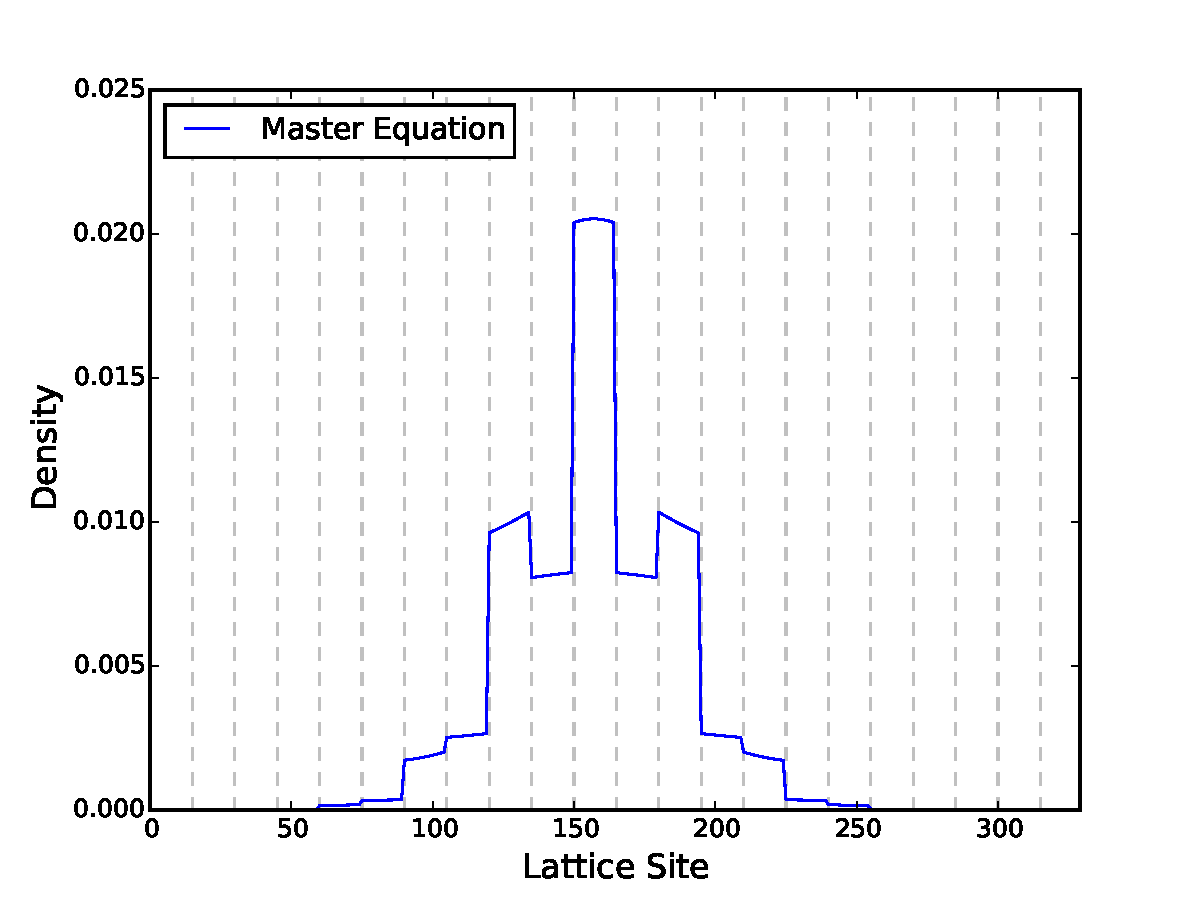
\includegraphics[width=1.0\linewidth]{../images/1D/11U_heterogeneous_plots_1D_nonphysical}
		\caption{1D heterogeneous system with internal semi-permeable boundaries. Non-physical density distribution simulated by violating the semi-permeable boundary condition (sometimes known as the isothermal boundary condition). Parameter specifications: 330 lattice sites, 15 lattice sites per cellular or extracellular region, $ D_i = 0.05 $, $ D_e = 0.2 $, and $ P_{i\rightarrow e} = 0.01 $ and $ P_{e\rightarrow i} =  0.005 $. Correctly chosen, $ P_{e\rightarrow i} =  0.0025 $. Vertical dashed lines show semi-permeable boundary positions. }
		\label{fig:11U_heterogeneous_plots_1D_nonphysical}
	\end{figure}
	
	\newpage
	Figure \ref{fig:11U_heterogeneous_plots_1D_nonphysical} shows the necessity of having coupled transition probabilities for the semi-permeable boundaries. The distribution in the long-time limit does not approach a uniform distribution, as would be expected for any system with passive semi-permeable boundaries and reflecting absolute boundaries. In the long-time, the density grows in certain cells and shrinks in others, similar to what might be expected if the semi-permeable boundaries behaved in an active-selective manner. 
	
	Section \ref{sec:1D-boundary-transition-probabilities} explores the effects of changing the semi-permeable boundary transition probability while maintaining region diffusivities constant. The second and last section \ref{sec:1D-cellular-extracellular-diffusivities} explores the effects of changing the ratio of the cellular and extracellular (C/EC) diffusivities while maintaining the semi-permeable boundary transition probability constant. In both sections and for all simulations, the size of the unit cell was constant, and C/EC regions were of the same dimensions.
	
\subsection{Boundary Transition Probabilities}
\label{sec:1D-boundary-transition-probabilities}
	The total transition probability is the product of two probabilities; the probability that a particle steps towards a boundary and the transition probability. The transition probability $ P_{i \rightarrow e} $ (``pie" in figure) is specified but the corresponding probability  $ P_{e \rightarrow i} $ can be easily calculated since the probabilities are coupled. For each plot, a different transition probability tested while all other parameters were held constant.
	
	\begin{figure}[h!]
		\centering
		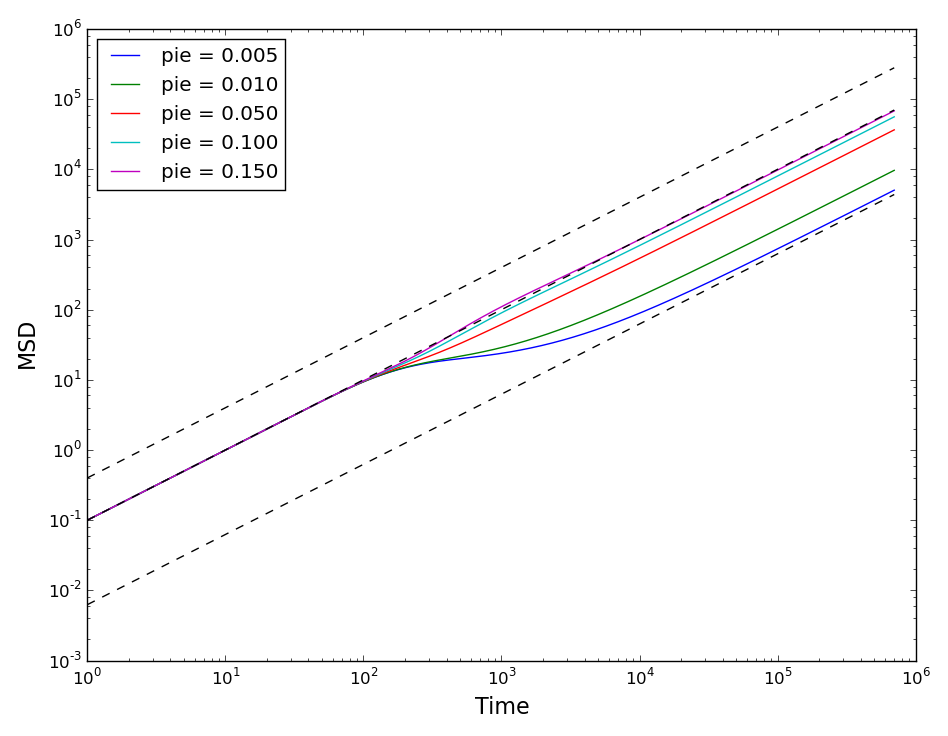
\includegraphics[width=1.0\linewidth]{../images/1D/pie_msd_1D}
		\caption{MSD versus time for 1D heterogeneous system. Parameter specifications: 3330 lattice sites, 15 lattice sites per cellular or extracellular region, $ D_i = 0.05 $, $ D_e = 0.2 $, and simulation time is $ 7\cdot 10^5 $ time steps. $ D = 0.2 $ for top dashed line, $ D = 0.05 $ for middle dashed line, and $ D = 0.5 \cdot (P_{i \rightarrow e} + P_{e \rightarrow i}) $ for the bottom dashed line (an average of the transition probabilities).}
		\label{fig:pie_msd_1D}
	\end{figure}
	
	 In Figure \ref{fig:pie_msd_1D}, the slope is clearly not unity for all time, for most of the plots, indicating the presence of anomalous diffusion. With decreasing transition probability, the magnitude of deviation from steady diffusion increases. Interestingly, for the largest transition probability simulated ($ P_{i \rightarrow e} = 0.150 $), the magnitude of deviation from steady diffusion is very small. It may be possible that for large transition probabilities, as long as the semi-permeable boundary transition condition is respected, approximately steady diffusion occurs for all time. In the long-time, the diffusion process becomes steady again for all transition probabilities tested. 
	 
	 In Figure \ref{fig:pie_beta_deff_1D}, the extent of the anomalous diffusion is clear in the $ \beta (t) $ versus $ t $ top figure. For all transition probabilities, steady diffusion occurs from the start of the simulation to some time where particles meet the semi-permeable boundary; this occurs at the same time for all simulations since C/EC diffusivity was constant. Both the magnitude of sub-diffusive behaviour and length of time before reaching steady diffusion, increase with decreasing transition probability. Super-diffusive behaviour appears only for two transition probabilities; it might be interesting to find the threshold transition probability that results in super-diffusive behaviour.
	 
	 In the bottom figure, the effective diffusivity may approach an average of the boundary transition probabilities, at least for transition probabilities much smaller than C/EC diffusivities. This is shown for $ P_{i \rightarrow e} = 0.150 $ and is observed for the other transition probabilities as well; however, this `average approach' sometimes under- or over-estimates the effective diffusivity obtained in the simulations and does not work well for transition probabilities approaching C/EC diffusivities, which may indicate dependence on regional diffusivities.
	
	\begin{figure}[h!]
		\centering
		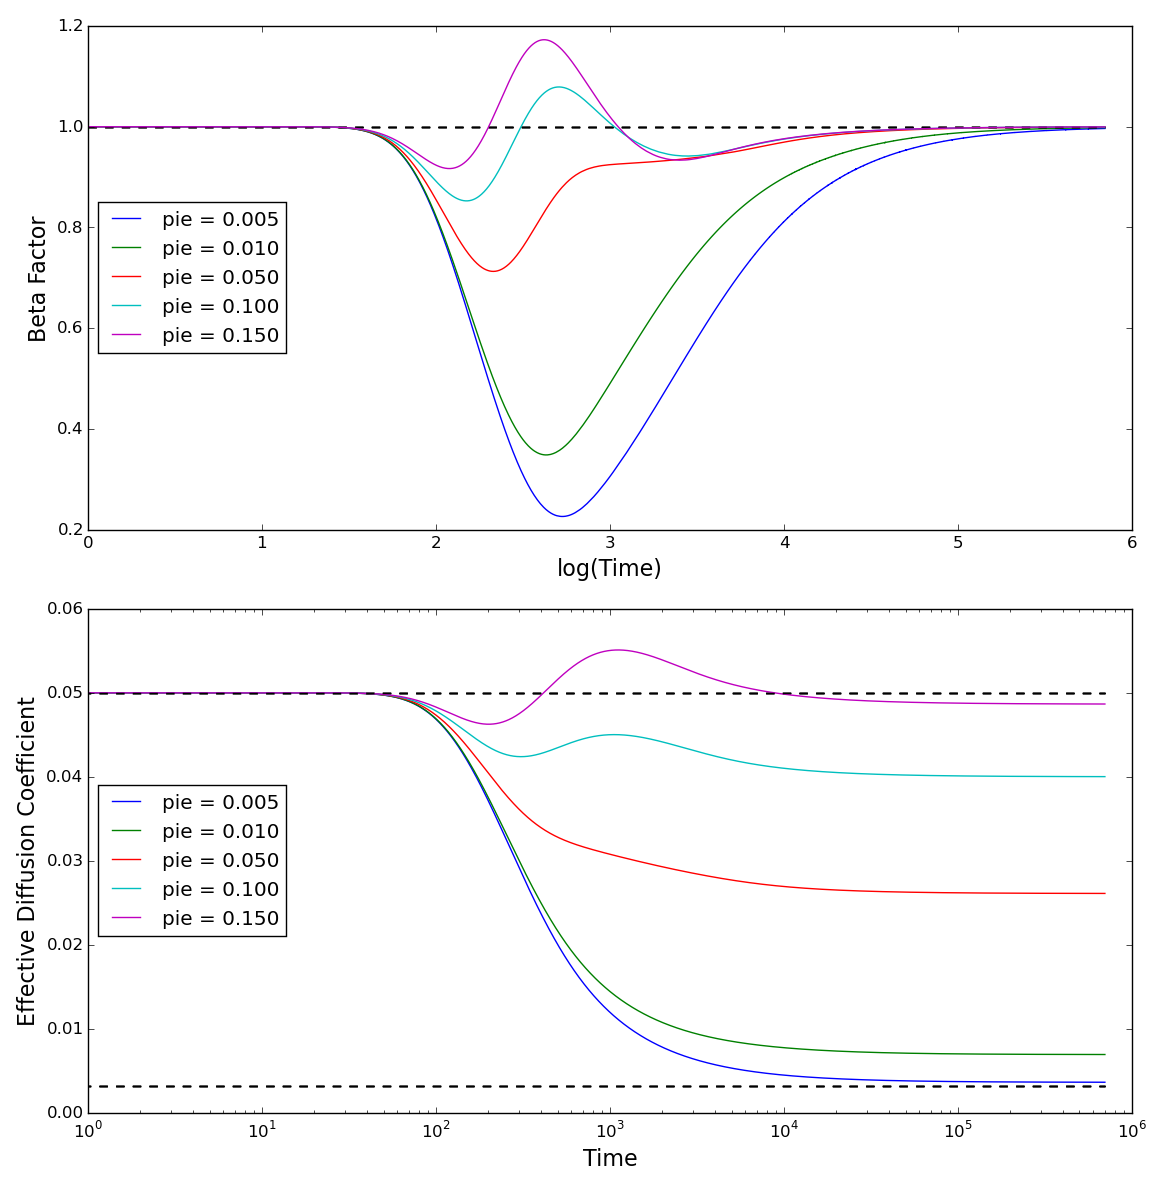
\includegraphics[width=1.0\linewidth]{../images/1D/pie_beta_deff_1D}
		\caption{$ \beta (t) $ versus log(time) and $ D_\textrm{eff} $ versus time for 1D heterogeneous system. Parameter specifications: 3330 lattice sites, 15 lattice sites per cellular or extracellular region, $ D_i = 0.05 $, $ D_e = 0.2 $, and simulation time is $ 7\cdot 10^5 $ time steps. In the lower figure, $ D = 0.05 $ for the upper dashed line and $ D = 0.5 \cdot (P_{i \rightarrow e} + P_{e \rightarrow i}) $ for the lower dashed line (an average of the transition probabilities).}
		\label{fig:pie_beta_deff_1D}
	\end{figure}

\clearpage
\subsection{Cellular and Extracellular Diffusivities}
\label{sec:1D-cellular-extracellular-diffusivities}
	For each plot, the ratio of cellular to extracellular diffusivities (indicated as ``pi/pe" on the figures), while all other parameters were held constant. More specifically, the cellular diffusivity was varied while the extracellular diffusivity was constant.
	
	\begin{figure}[h!]
		\centering
		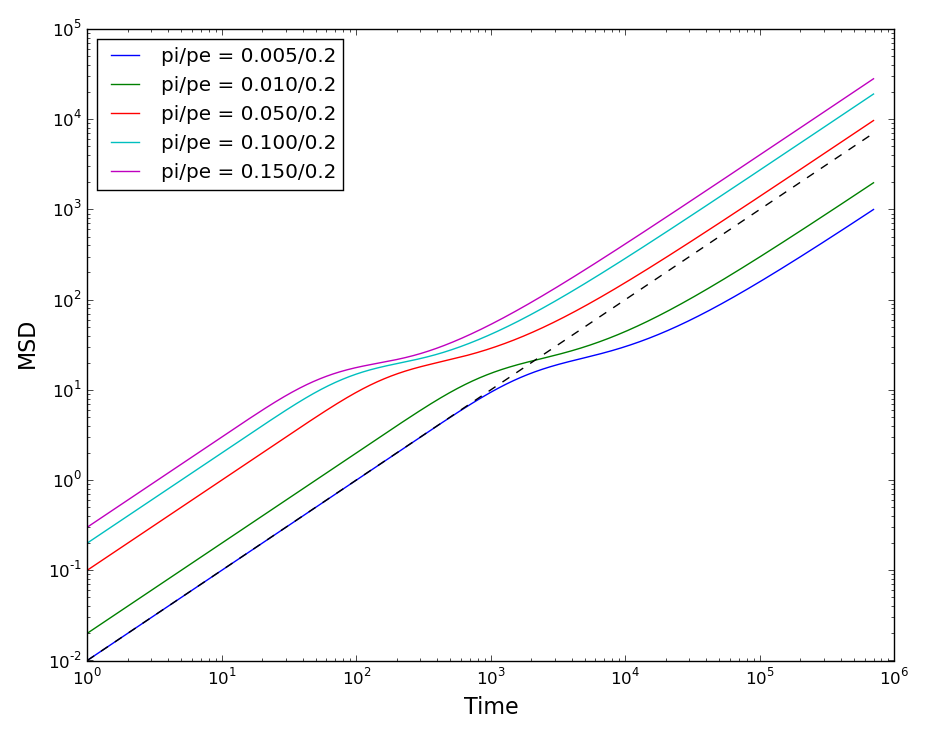
\includegraphics[width=1.0\linewidth]{../images/1D/pipe_msd_1D}
		\caption{MSD versus time for 1D heterogeneous system. Parameter specifications: 3330 lattice sites, 15 lattice sites per cellular or extracellular region, $ P_{i \rightarrow e} = 0.01 $, and simulation time is $ 7\cdot 10^5 $ time steps. $ D = 0.005 $ for the dashed line.}
		\label{fig:pipe_msd_1D}
	\end{figure}
	
	In Figure \ref{fig:pipe_msd_1D}, anomalous diffusion is observed for all diffusivity ratios and in particular, no super-diffusive behaviour occurs. This last point is clearly evident in Figure \ref{fig:pipe_beta_deff_1D}; none of the ratios tested result in $ \beta > 1 $ for any time. The displacement of the peak of the curves in time is due to the varying cellular diffusivities tested. The larger the diffusivity of the region in which the particles start, the quicker the particles reach the semi-permeable boundary and sub-diffusive behaviour occurs. Interestingly, the magnitude in the deviation from steady diffusion is approximately the same for all C/EC diffusivity ratios. 
	
	The effective diffusion in the long-time is non-trivial; it does not seem to approach some derivable value. It likely depends on the C/EC diffusivities and transition probabilities but the relationship is not obvious. All that can be said for now is qualitative; for every C/EC diffusivity ratio tested, the effective diffusivity in the long time is less than the starting region diffusivity and the larger the starting diffusivity, the greater the difference from the long-time effective diffusivity. For ratios close to unity and transition probabilities very small, the effective diffusion coefficient may approach the average of the transition probabilities but this cannot be said with certainty. Further testing is needed.
	
	\begin{figure}[h!]
		\centering
		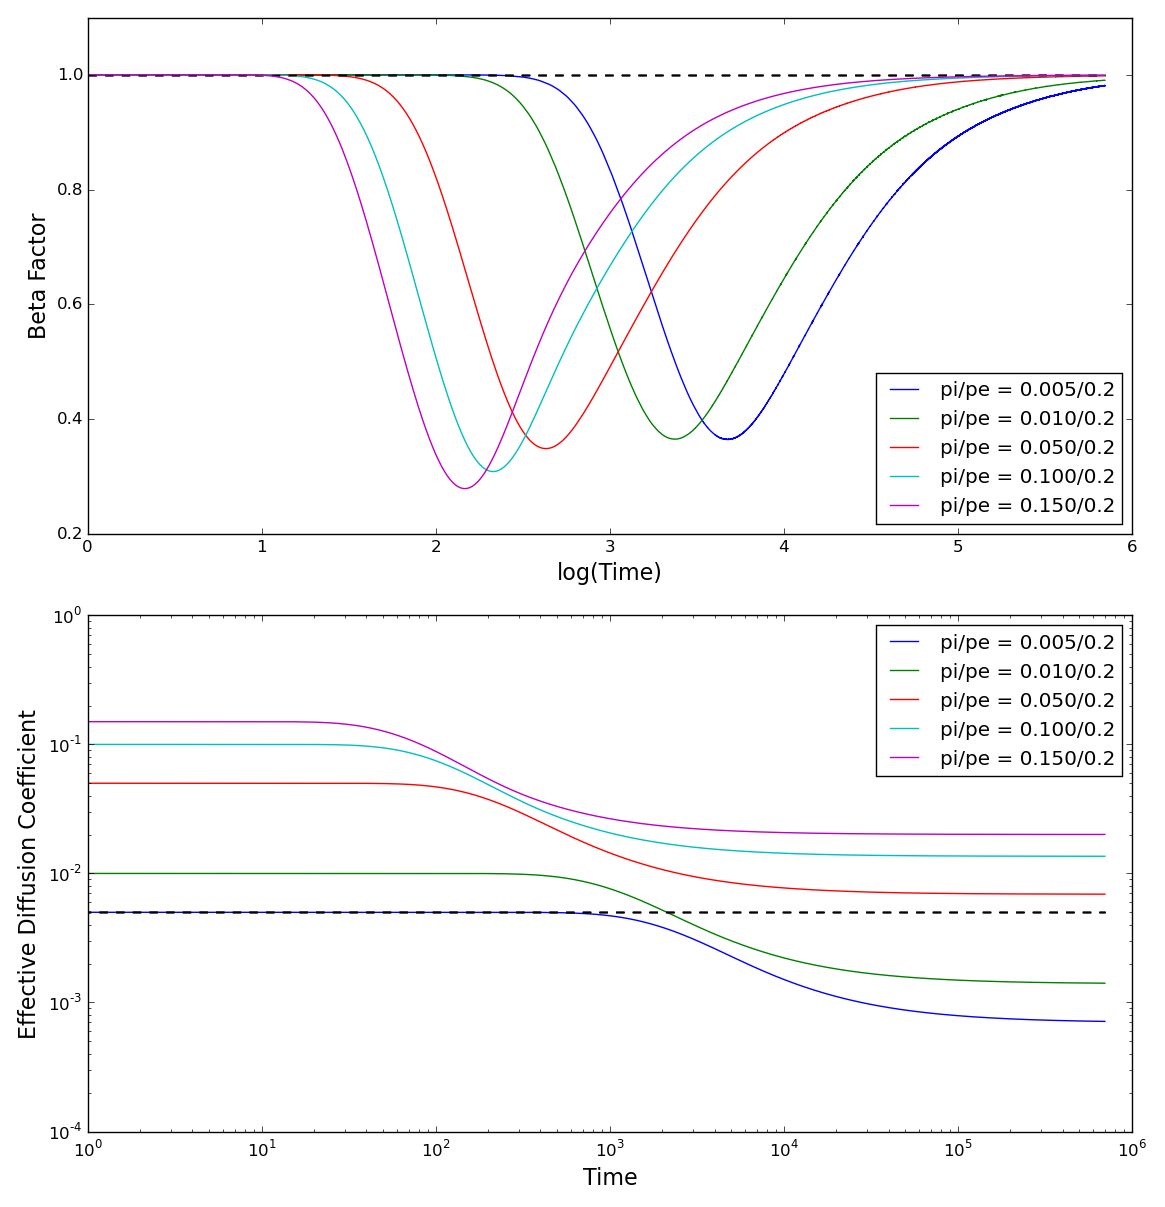
\includegraphics[width=1.0\linewidth]{../images/1D/pipe_beta_deff_1D}
		\caption{$ \beta (t) $ versus log(time) and $ D_\textrm{eff} $ versus time for 1D heterogeneous system. Parameter specifications: 3330 lattice sites, 15 lattice sites per cellular or extracellular region, $ P_{i \rightarrow e} = 0.01 $, and simulation time is $ 7\cdot 10^5 $ time steps. In the lower figure, $ D = 0.005 $ for the dashed line.}
		\label{fig:pipe_beta_deff_1D}
	\end{figure}

\clearpage
\section{2D Systems}
\label{sec:ra-2D}
	The analysis of 2D systems proceeded in the same manner as for 1D systems, except with the addition of another variable for testing: extracellular channel width. Section \ref{sec:2D-boundary-transition-probabilities} explores the effects of changing the semi-permeable boundary transition probability while maintaining C/EC diffusivities and channel width, constant. The second section \ref{sec:2D-cellular-extracellular-diffusivities} explores the effects of changing the ratio of the C/EC diffusivities while maintaining the semi-permeable boundary transition probabilities and channel width, constant. The third and final section \ref{sec:2D-channel-width} explores the effects of changing the width of the extracellular channel in $ \hat{y} $ while maintaining the ratio of C/EC diffusivities and semi-permeable boundary transition probabilities, constant.
	
	The 2D system is divided into two halves, upper and lower. The upper halve consists of alternating cellular and extracellular regions of the same and square geometry; the dimensions of these regions were the same for every simulation. The lower halve consists of a single extracellular channel.
	
	Due to the computational time required to simulate using MC, all simulations used for analysis were ME simulations and because of the additional physical dimension, more particles are needed in the MC simulation to obtain smoother distributions with smaller fluctuations. Figure \ref{fig:heterogeneous_3U_2D} and \ref{fig:MC_heterogeneous_3U_2D} show `heat maps' of the 2D density distribution at the same time step, for comparison. Figure \ref{fig:heterogeneous_11U_2D} shows diffusion in a larger system where particles have not reached the absolute boundaries and Figure \ref{fig:error_in_diffusion} shows a barely visible non-physical density distribution, created by purposely violating the ``iso-thermal" semi-permeable boundary condition.
	
	\begin{figure}[h]
		\centering
		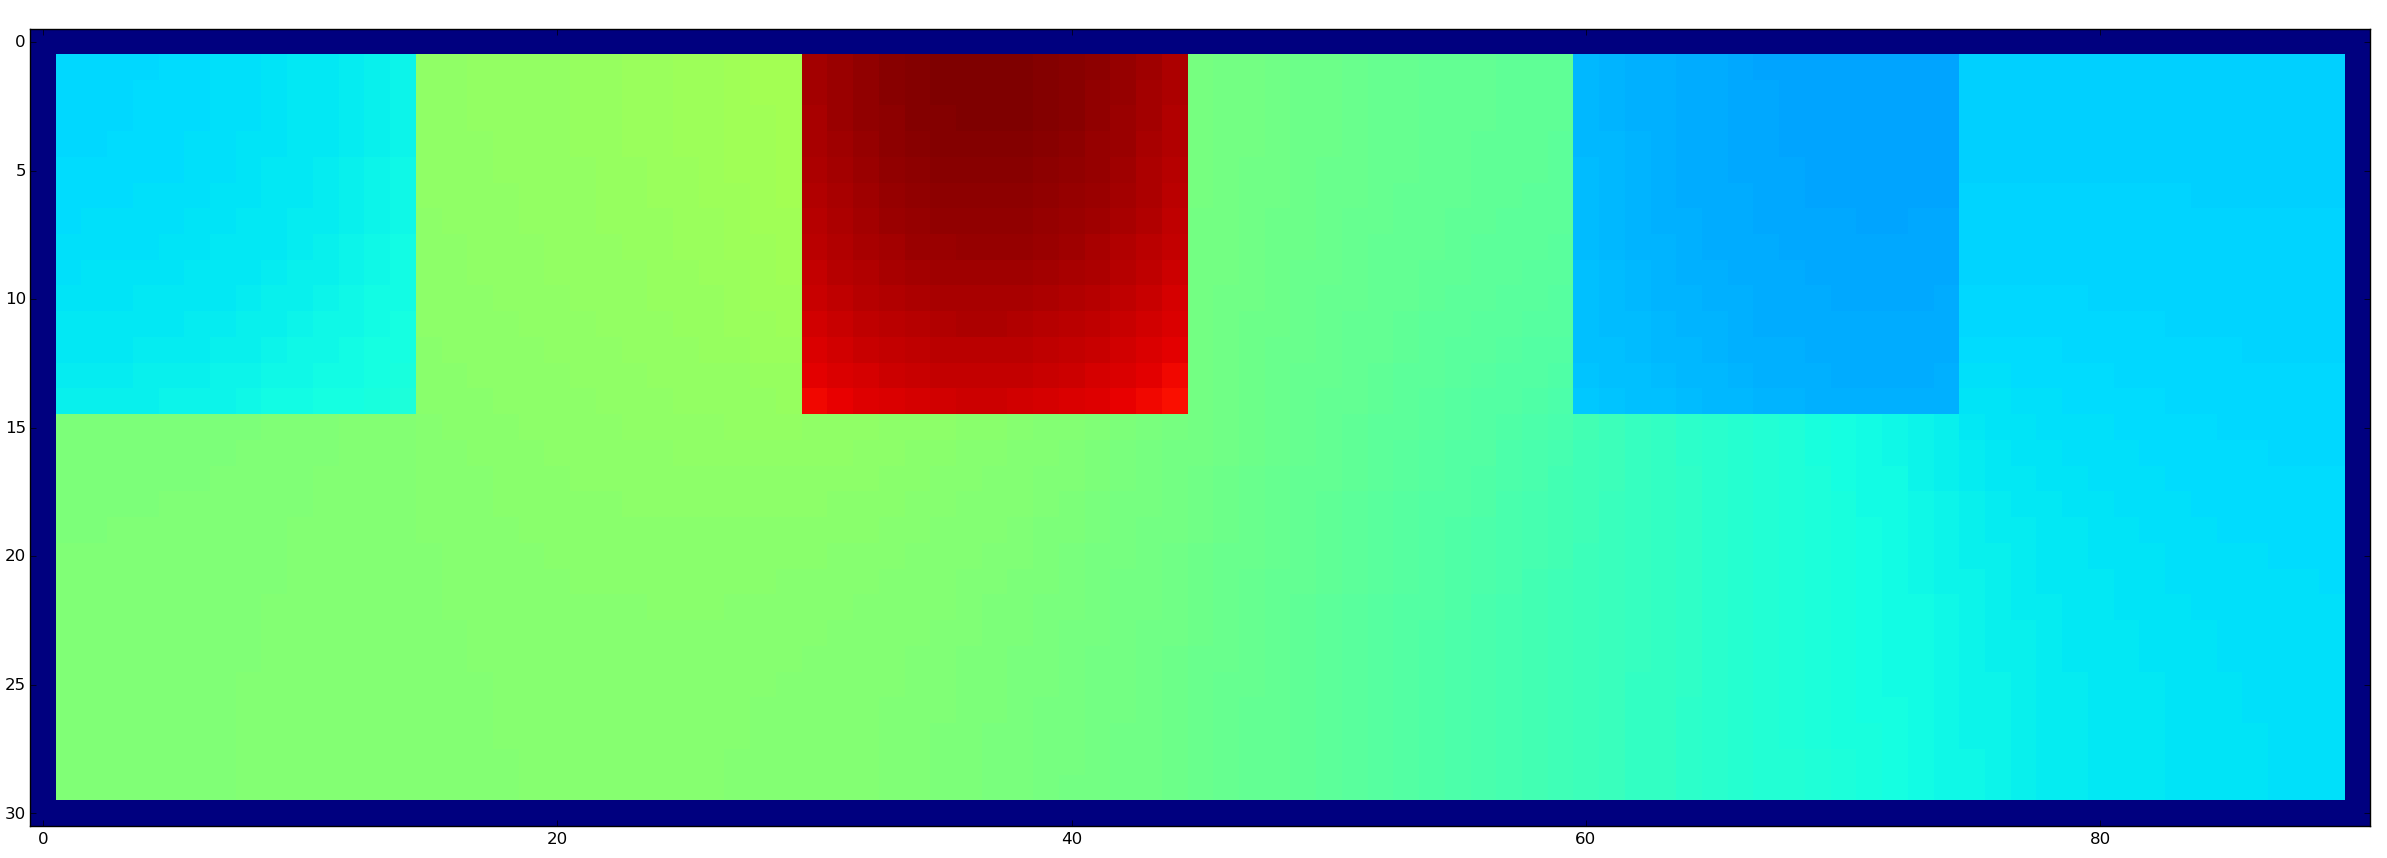
\includegraphics[width=1.0\linewidth]{../images/2D/heterogeneous_3U_2D}
		\caption{Master equation simulation of diffusion in a 2D heterogeneous system. Parameter specifications: 90 lattice sites in $ \hat{x} $ and 30 lattice sites in $ \hat{y} $, ($ 15 \times 15 $) lattice sites per cellular or extracellular region, $ D_i = 0.05 $, $ D_e = 0.2 $, and $ P_{i\rightarrow e} = 0.025 $. Semi-permeable boundaries are clearly visible.}
		\label{fig:heterogeneous_3U_2D}
	\end{figure}
	
	\begin{figure}[h!]
		\centering
		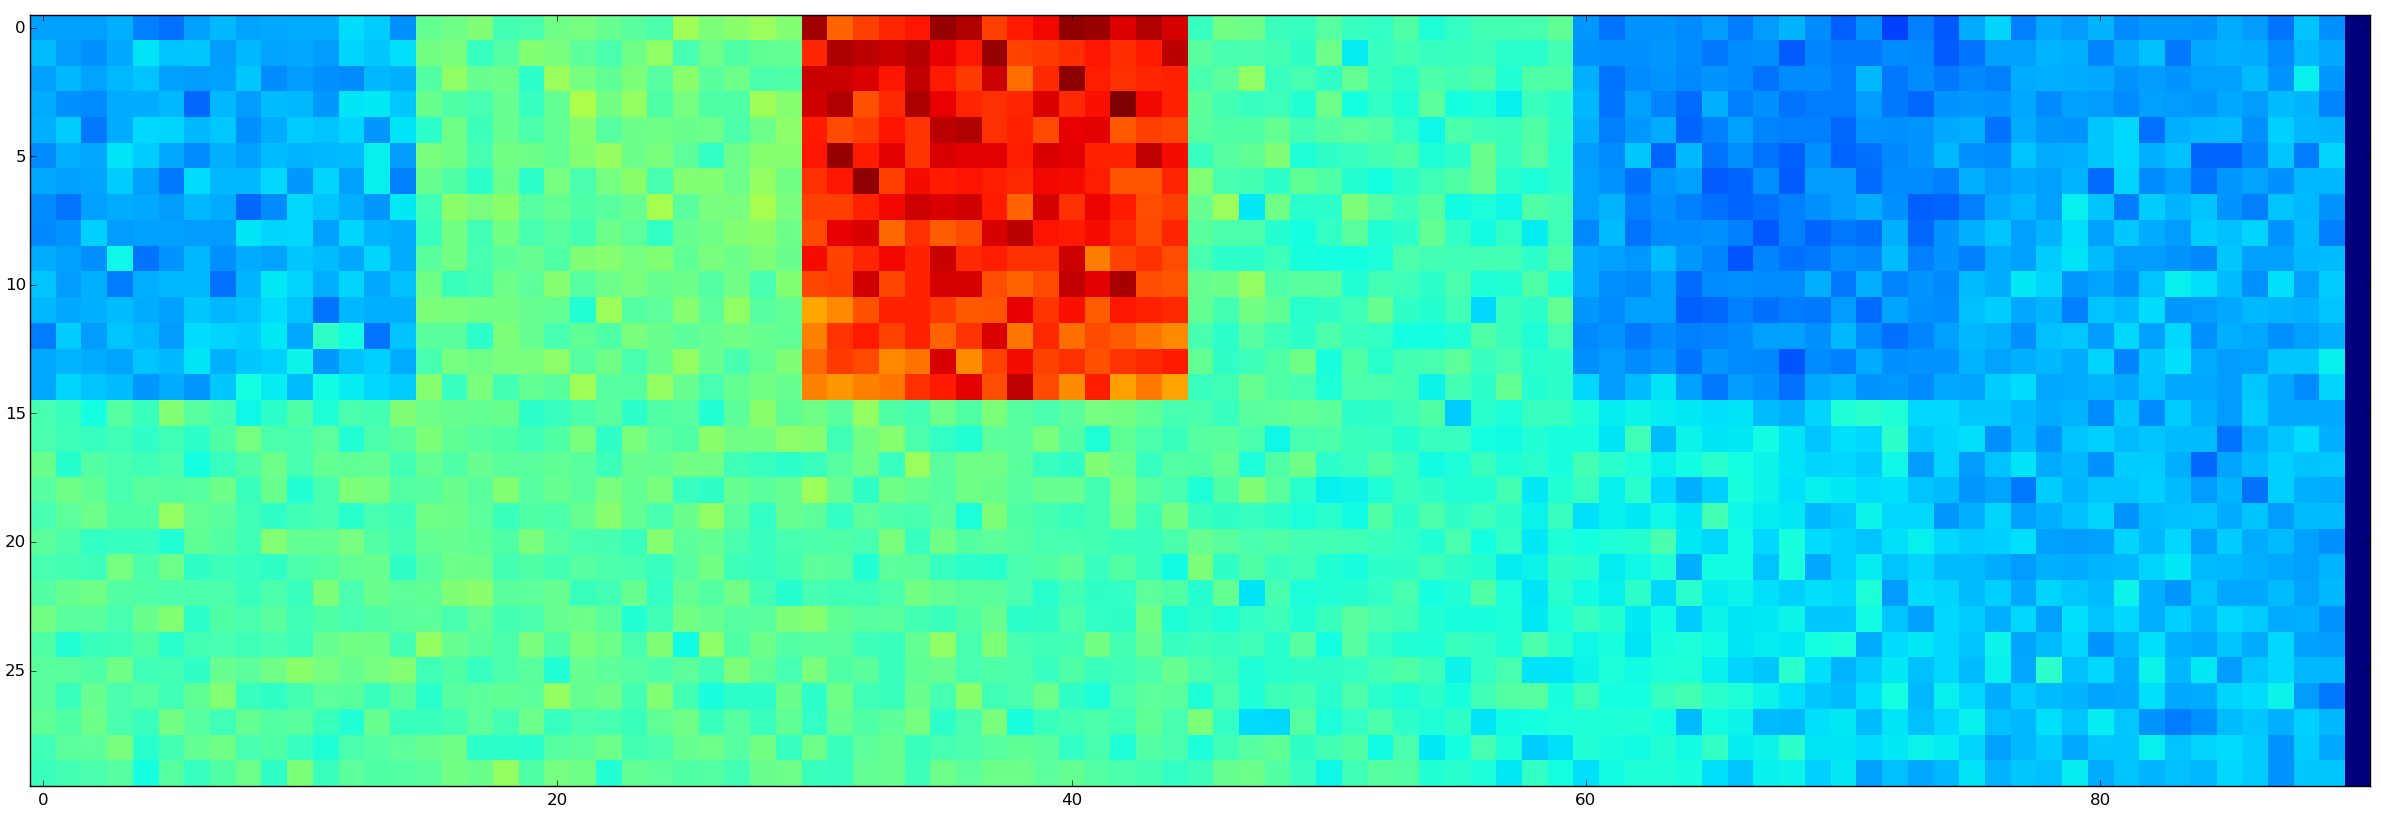
\includegraphics[width=1.0\linewidth]{../images/2D/MC_heterogeneous_3U_2D}
		\caption{Monte Carlo simulation of diffusion in a 2D heterogeneous system. Parameter specifications: 90 lattice sites in $ \hat{x} $ and 30 lattice sites in $ \hat{y} $, ($ 15 \times 15 $) lattice sites per cellular or extracellular region, $ D_i = 0.05 $, $ D_e = 0.2 $, and $ P_{i\rightarrow e} = 0.025 $, $ N = 5 \cdot 10^5 $ particles used.}
		\label{fig:MC_heterogeneous_3U_2D}
	\end{figure}
	
	\begin{figure}[h!]
		\centering
		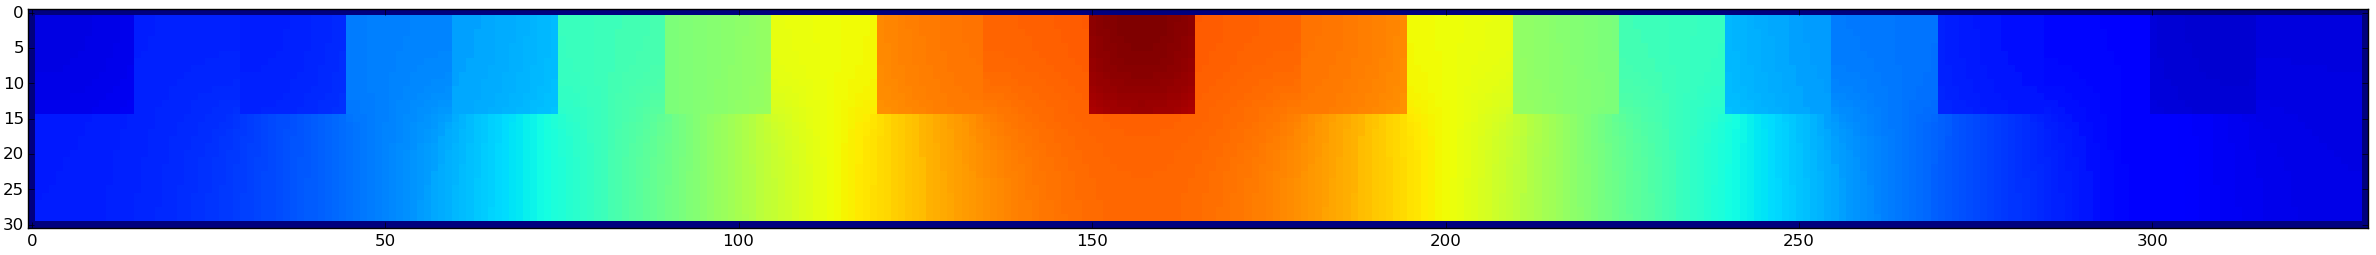
\includegraphics[width=1.0\linewidth]{../images/2D/heterogeneous_11U_2D}
		\caption{Master equation simulation of diffusion in a larger 2D heterogeneous system. Parameter specifications: 90 lattice sites in $ \hat{x} $ and 330 lattice sites in $ \hat{y} $, ($ 15 \times 15 $) lattice sites per cellular or extracellular region, $ D_i = 0.05 $, $ D_e = 0.2 $, and $ P_{i\rightarrow e} = 0.025 $, $ N = 5 \cdot 10^5 $ particles used.}
		\label{fig:heterogeneous_11U_2D}
	\end{figure}
	
	\begin{figure}[h!]
		\centering
		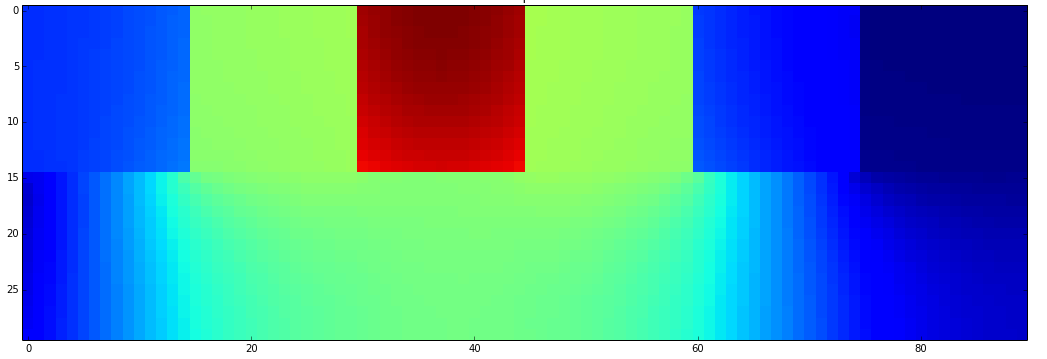
\includegraphics[width=1.0\linewidth]{../images/2D/error_in_diffusion}
		\caption{Master equation simulation of diffusion in 2D heterogeneous system. Non-physical density distribution simulated by violating the semi-permeable boundary condition. Note the slightly visible `boundary' edges separating the upper extracellular region from lower extracellular channel. Errors may be less perceivable than in the 1D simulations and will likely not be visible until many time steps have elapsed and/or the system is very small.}
		\label{fig:error_in_diffusion}
	\end{figure}

\newpage
\subsection{Boundary Transition Probabilities}
\label{sec:2D-boundary-transition-probabilities}

	For all transition probabilities tested (``pie" in figures), anomalous diffusion behaviour is present. Inspection of the MSD versus time plots in Figure \ref{fig:pie_msd_2D}, shows initial sub-diffusive behaviour caused by particles meeting semi-permeable boundary of the starting region, followed by super-diffusive behaviour as particles exit their initial enclosure and reach the high-diffusivity extracellular region.  Note that a single MC simulation was run with the same parameters as the corresponding ME simulation. The two are in good agreement but $ D_\textrm{eff} $ calculated from the MC simulation is slightly smaller than calculated from the ME simulation, beyond a time where most particles have left the starting region. This discrepancy may by due to the finite number of particles used and the statistical error introduced by low particle densities.
	
	\begin{figure}[h!]
		\centering
		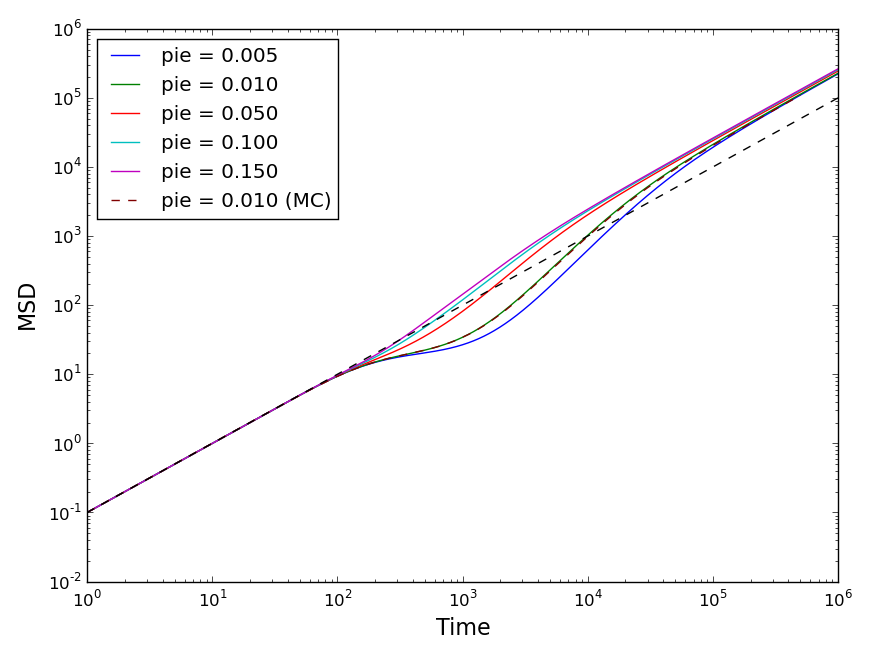
\includegraphics[width=1.0\linewidth]{../images/2D/pie_msd_2D}
		\caption{MSD versus time for 2D heterogeneous system. Parameter specifications: 3630 lattice sites, 15 lattice site channel width, ($ 15 \times 15 $) lattice sites per cellular or extracellular region, $ D_i = 0.05 $, $ D_e = 0.2 $, and simulation time is $ 10^6 $ time steps. $ D = 0.05 $ for the dashed line.}
		\label{fig:pie_msd_2D}
	\end{figure}
	
	In Figure \ref{fig:pie_beta_deff_2D}, similar to the 1D case, the magnitude of the deviation from steady diffusion decreases with increasing transition probability, except now there is also super-diffusive behaviour present due to the extracellular channel. Observe the diffusive behaviour in the case of $ P_{i \rightarrow e}  = 0.150 $, there is a temporary plateau where the magnitude of super-diffusive behaviour is constant for some interval of time. Interestingly, in the $ \beta $ versus $ \log(t) $ plot, the time difference between the maximum and minimum of each plot increases with decreasing transition probability. Essentially, the time spent in anomalous diffusion by a system increases with decreasing transition probability.
	
	The effective diffusivity in the long-time is non-trivial and its dependence on the boundary transition probabilities, C/EC diffusivity ratios, and channel geometry is not obvious.
	
	\begin{figure}[h!]
		\centering
		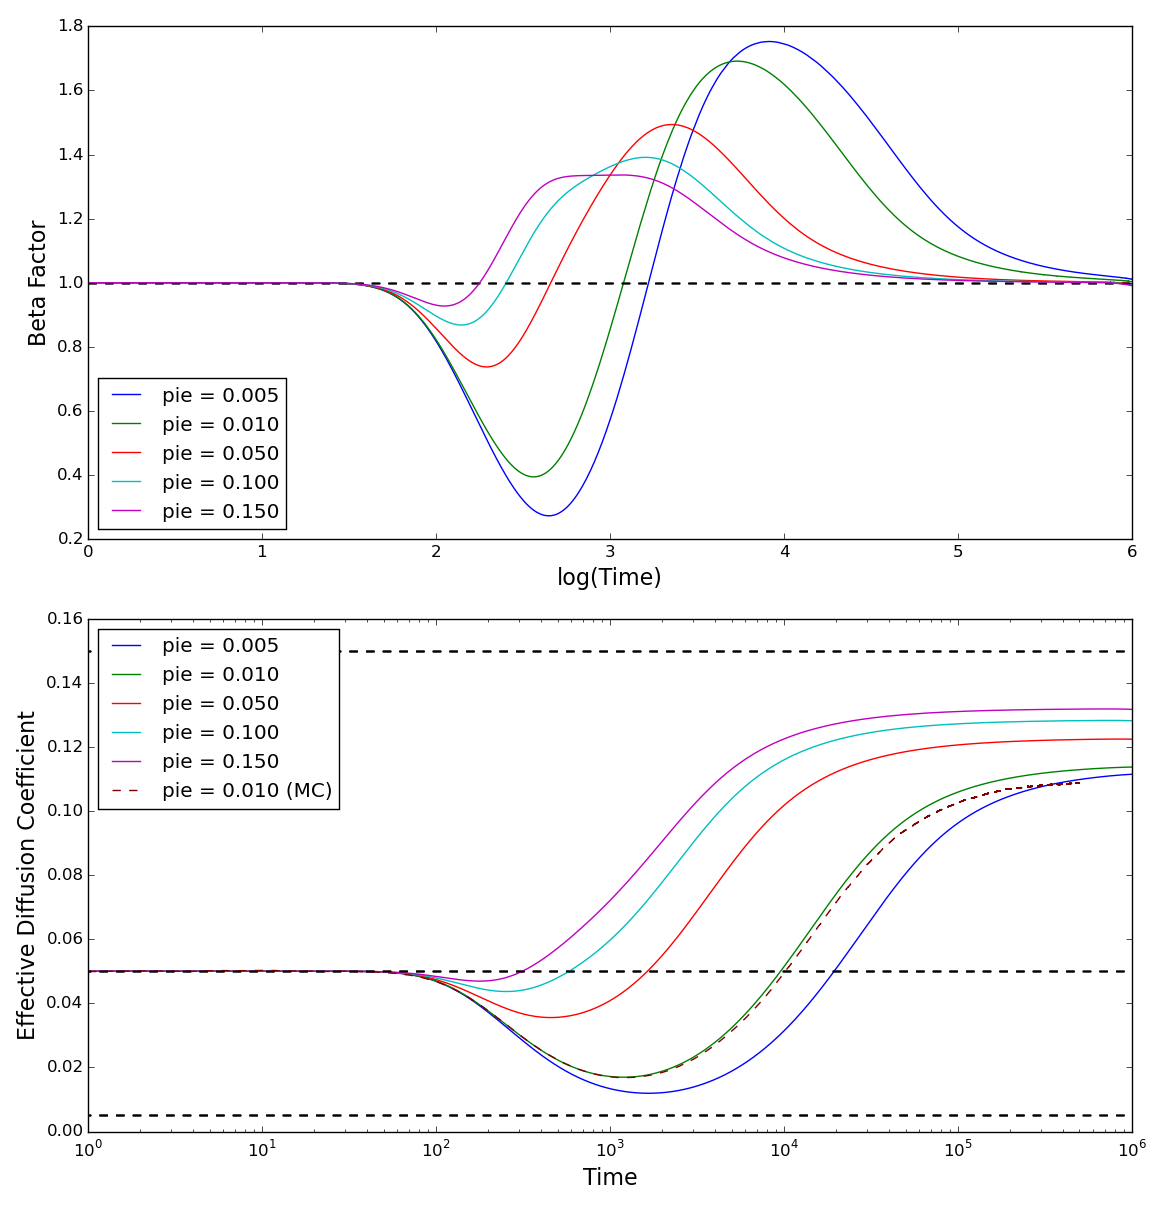
\includegraphics[width=1.0\linewidth]{../images/2D/pie_beta_deff_2D}
		\caption{$ \beta (t) $ versus log(time) and $ D_\textrm{eff} $ versus time for 2D heterogeneous system. Parameter specifications: 3630 lattice sites, 15 lattice site channel width, ($ 15 \times 15 $) lattice sites per cellular or extracellular region, $ D_i = 0.05 $, $ D_e = 0.2 $, and simulation time is $ 10^6 $ time steps. In the lower figure, $ D = 0.15 $ for the top dashed line and $ D = 0.05 $ for the middle dashed line, and $ D = 0.005 $ for the bottom dashed line.}
		\label{fig:pie_beta_deff_2D}
	\end{figure}

\clearpage
\subsection{Cellular and Extracellular Diffusivities}
\label{sec:2D-cellular-extracellular-diffusivities}	
	
	For all ratios of C/EC diffusivity tested (``pi/pe" in figures), it appears that regardless of the diffusivity of the starting region, the long-time effective diffusion coefficients are nearly the same.
	
	\begin{figure}[h]
		\centering
		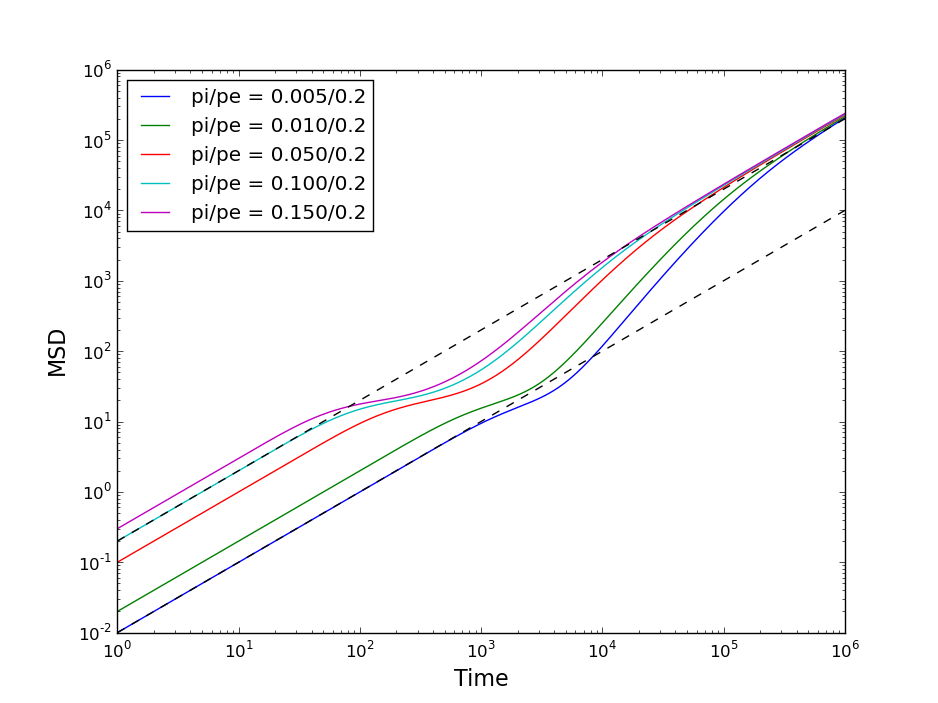
\includegraphics[width=1.0\linewidth]{../images/2D/pipe_msd_2D}
		\caption{MSD versus time for 2D heterogeneous system. Parameter specifications: 3030 lattice sites, 15 lattice site channel width, ($ 15 \times 15 $) lattice sites per cellular or extracellular region, $ D_e = 0.2 $, $ P_{i \rightarrow e} = 0.01 $, and simulation time is $ 10^6 $ time steps. $ D = 0.1 $ for the upper dashed line and $ D = 0.005 $ for the lower dashed line.}
		\label{fig:pipe_msd_2D}
	\end{figure}
	
	Compared to the 1D simulations where only sub-diffusive behaviour was observed, sub- and super-diffusive behaviour is observed for all C/EC ratios tested, in the 2D simulations. The displacement in the minimum of each plot in Figure \ref{fig:pipe_beta_deff_2D} is characteristic of different diffusivities in the particle's starting region.
	
	The long-time effective diffusion coefficients appear to converge to the same value, but it is unclear how this value depends on the parameters tested and it is unknown how changing other parameters might affect this long-time value. It might be interesting to test how the long-time effective diffusion coefficient depends on specific values of $ D_i $ and $ D_e $, while maintaining the ratio of these values constant.
	
	\begin{figure}[h!]
		\centering
		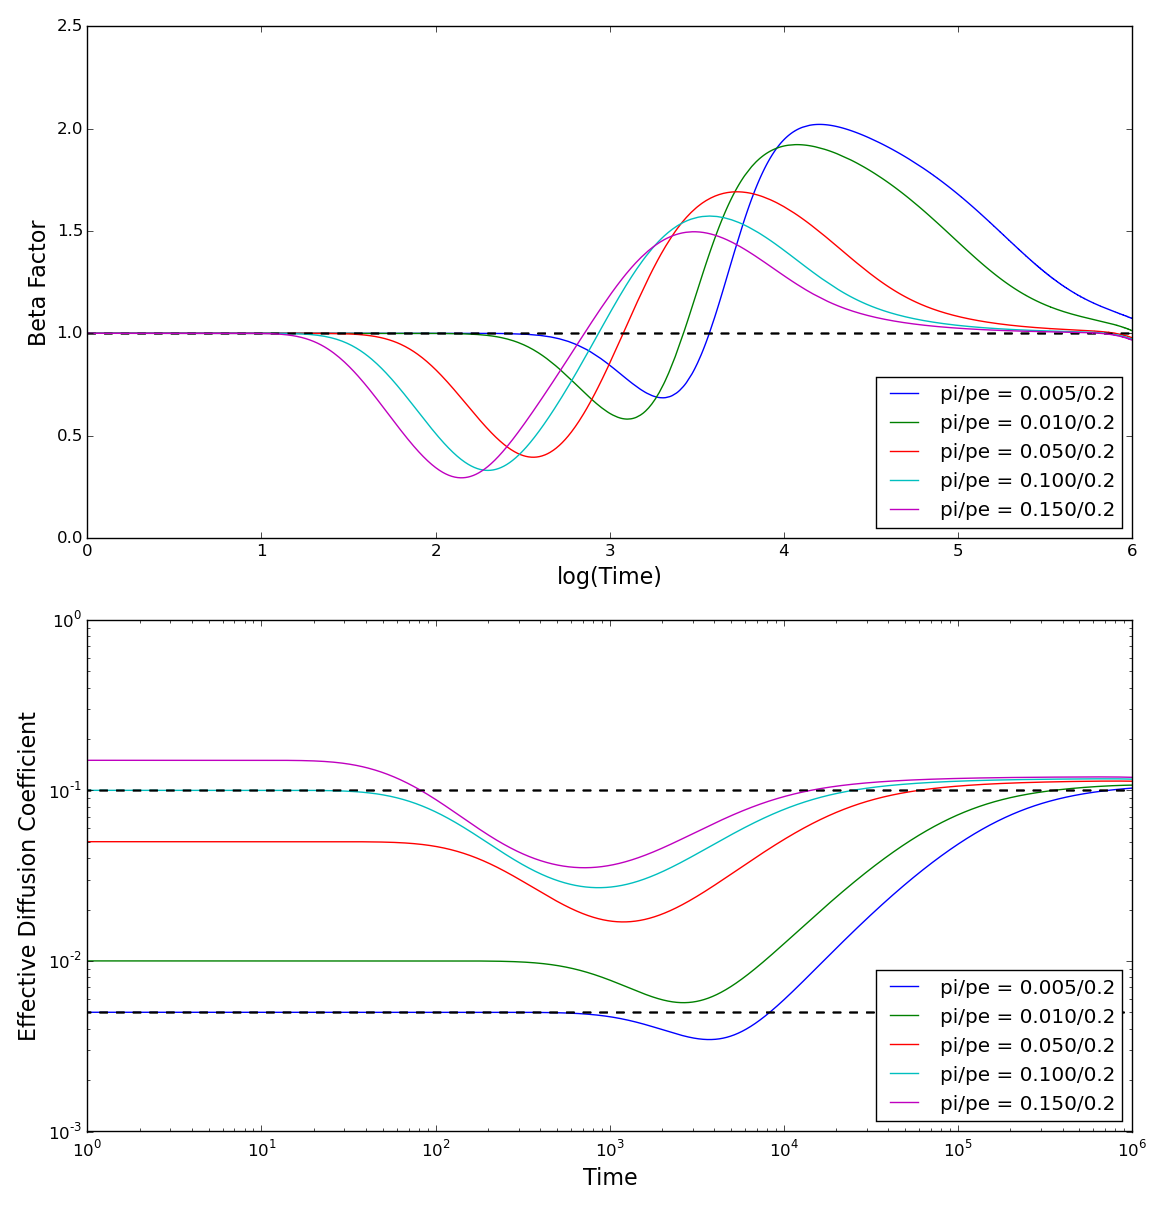
\includegraphics[width=1.0\linewidth]{../images/2D/pipe_beta_deff_2D}
		\caption{$ \beta (t) $ versus log(time) and $ D_\textrm{eff} $ versus time for 2D heterogeneous system. Parameter specifications: 3030 lattice sites, 15 lattice site channel width, ($ 15 \times 15 $) lattice sites per cellular or extracellular region, $ D_e = 0.2 $, $ P_{i \rightarrow e} = 0.01 $, and simulation time is $ 10^6 $ time steps. In the lower figure, $ D = 0.1 $ for the upper dashed line and $ D = 0.005 $ for the lower dashed line.}
		\label{fig:pipe_beta_deff_2D}
	\end{figure}
	
\clearpage
\subsection{Extracellular Channel Widths}
\label{sec:2D-channel-width}
	
	The extracellular channel may be used as a `conduit' for particles and it is possible that once leaving the initial enclosure, a particle may not interact with a semi-permeable boundary. Therefore, how the dimensions of this channel affect diffusive behaviour and the long-time effective diffusion coefficient are of interest. The standard channel width for all other simulations was 15 lattice units. A channel width of 0 lattice units was also tested in order to simulate a pseudo-1D system. 
	
	\begin{figure}[h]
		\centering
		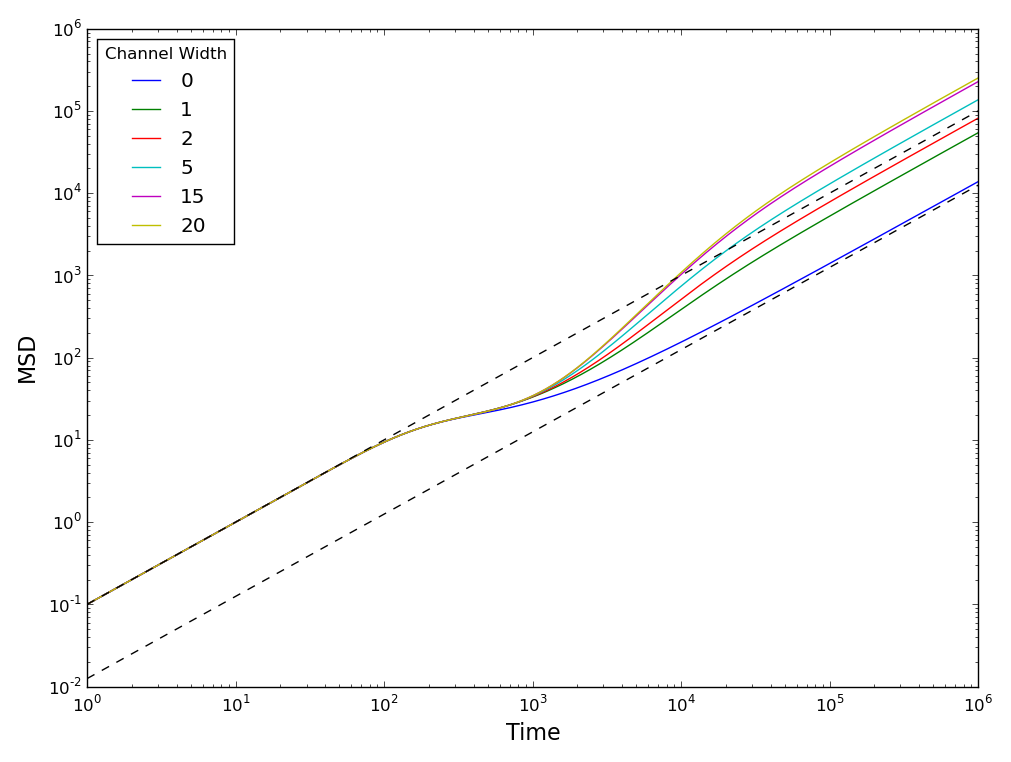
\includegraphics[width=1.0\linewidth]{../images/2D/ye_msd_2D}
		\caption{MSD versus time for 2D heterogeneous system. Parameter specifications: 3030 lattice sites, ($ 15 \times 15 $) lattice sites per cellular or extracellular region, $ D_i = 0.05 $, $ D_e = 0.2 $, $ P_{i \rightarrow e} = 0.01 $, and simulation time is $ 10^6 $ time steps.}
		\label{fig:ye_msd_2D}
	\end{figure}
	
	Similar to the 1D system with the same diffusivity and transition probability parameters, only sub-diffusive behaviour occurred in the 2D system with no extracellular channel (refer to Figure \ref{fig:pie_msd_1D} and \ref{fig:pie_beta_deff_1D}). Observe in Figure \ref{fig:ye_beta_deff_2D}, the addition of even a single (1) lattice site as an extracellular channel results in super-diffusive behaviour. It appears the change in diffusion behaviour becomes less dramatic with increasing channel width. Larger channel widths need to be tested to verify this and identify how $ \beta $ might depend on channel width.
	
	It is not certain how the long-time effective diffusivity depends on the channel width and other parameters. What can be said is that increasing the width of the channel makes more of the highly diffusive extracellular space available for the particles, therefore it is expected that larger channel widths result in greater long-time effective diffusivities (up to a certain limit: the extracellular diffusivity).
	
	\begin{figure}[h]
		\centering
		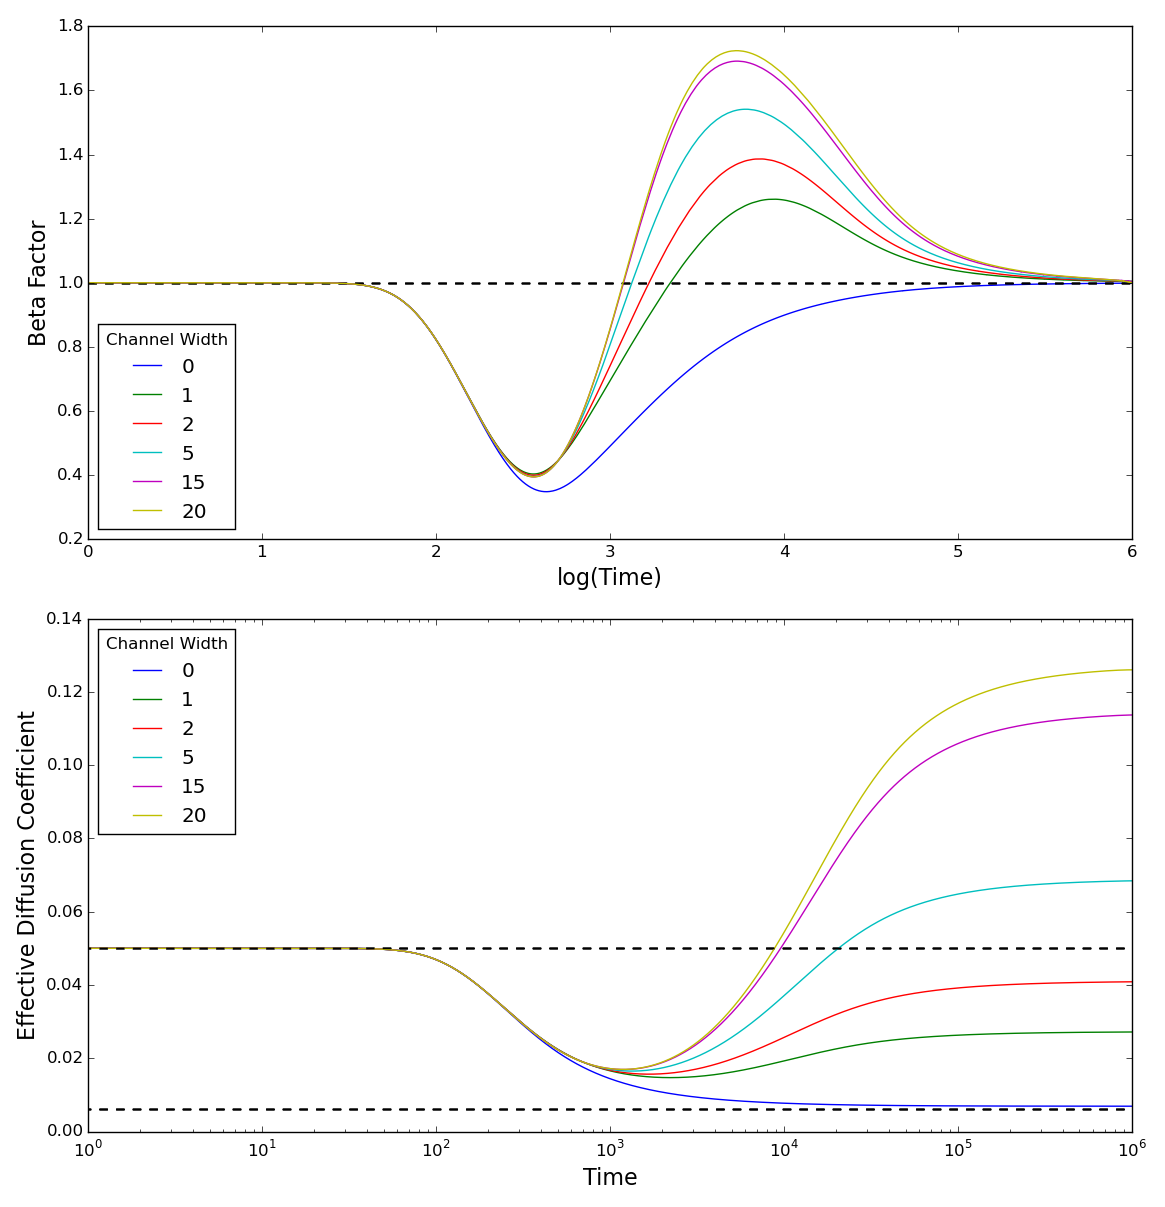
\includegraphics[width=1.0\linewidth]{../images/2D/ye_beta_deff_2D}
		\caption{$ \beta (t) $ versus log(time) and $ D_\textrm{eff} $ versus time for 2D heterogeneous system. Parameter specifications: 3030 lattice sites, ($ 15 \times 15 $) lattice sites per cellular or extracellular region, $ D_i = 0.05 $, $ D_e = 0.2 $, $ P_{i \rightarrow e} = 0.01 $, and simulation time is $ 10^6 $ time steps. In the lower figure, $ D = 0.05 $ for the upper dashed line and $ D = 0.5 \cdot (P_{i \rightarrow e} + P_{e \rightarrow i}) $ for the lower dashed line (an average of the transition probabilities, similar to the 1D case).}
		\label{fig:ye_beta_deff_2D}
	\end{figure}

	